\section{Analyse des communications et bilan de liaison}
\href{https://youtu.be/qFMQgfgPAvg}{Cliquer pour visuliser}
\begin{figure}[H]
    \centering
    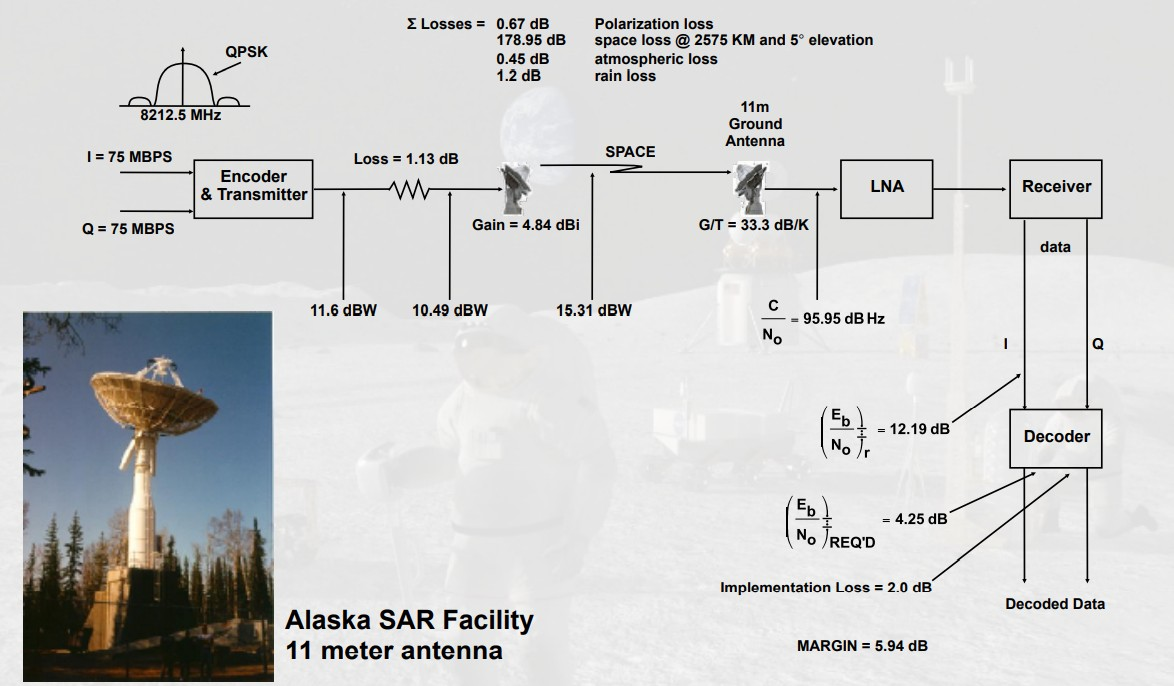
\includegraphics[width=0.8\textwidth]{figures/6-90.jpg}
    \caption{Un exemple de bilan de liaison sous forme de diagramme. Image du Dr Akin.}
    \label{fig:communication7}
\end{figure}

\noindent Vous aurez également besoin des informations suivantes, fournies par vous et votre client :

\begin{itemize}
    \item Latitude et longitude des stations terrestres de liaison montante et descendante.
    \item Débit de données ou d'informations prévu.
    \item Type de modulation (\textbf{BPSK} ou \textbf{QPSK}).
    \item Taux de correction d'erreur directe (\textbf{1/2} ou \textbf{3/4}).
    \item Facteur d'étalement (si applicable, pour les systèmes à spectre étalé).
    \item Fréquences de liaison montante et de liaison descendante.
    \item Tailles des antennes de liaison montante et descendante.
    \item Efficacité des antennes de liaison montante et descendante.
    \item Gains de transmission et de réception en liaison montante et descendante (exprimés en fréquence).
    \item Puissance minimale du signal numérique (\textbf{E\textsubscript{b}/N\textsubscript{o}}) pour garantir les performances souhaitées en termes de taux d'erreur binaire (\textbf{BER}).
\end{itemize}

Une fois ces informations disponibles, il suffit de saisir les données dans la feuille de calcul pour calculer le budget de liaison.

\medskip
\noindent \textbf{Calculateurs de budget de liaison pour un système de communication RF et optique :}
\begin{itemize}
    \item \href{https://www.satsig.net/linkbugt.htm}{satsig.net}
    \item \href{http://www.satcoms.org.uk/satellite-link-budget-calculator.asp}{satcoms.org.uk}
    \item \href{https://www.tutorialsweb.com/satcom/satellite-link-budget-calculator.htm}{tutorialsweb.com}
    \item \href{https://spacegrant.colorado.edu/COSGC_Projects/co3sat/downloads/CS1-COM100.03\%20AMSAT\%20IARU\%20Link\%20Budget.xls}{Colorado Space Grant}
    \item \href{https://cedarweb.vsp.ucar.edu/wiki/images/7/75/Cubesat_Link-Budget.xls}{Cubesat Link Budget}
    \item \href{https://www.maximintegrated.com/content/dam/files/design/tools/tech-docs/5142/AN5142-link-budget.xls}{Maxim Integrated}
    \item \href{https://www.rfwireless-world.com/downloads/RF-Link-Budget.xlsx}{RF Wireless World}
    \item \href{https://sourceforge.isae.fr/projects/satlinktool-a-tool-for-analysing-geo-satcom/wiki/Link_Budget}{SatLinkTool (ISAE)}
\end{itemize}
\noindent \textbf{Lectures suggérées :} 
\href{http://rfic.eecs.berkeley.edu/~niknejad/ee242/pdf-lock/NIST_LinkBudgetCalc_2_4_konglk.xls}{NIST Link Budget Calculator}

\medskip
\noindent \textbf{Activité suggérée :} 
Produire un budget de liaison.
